\begin{figure}[h]
 \centering
 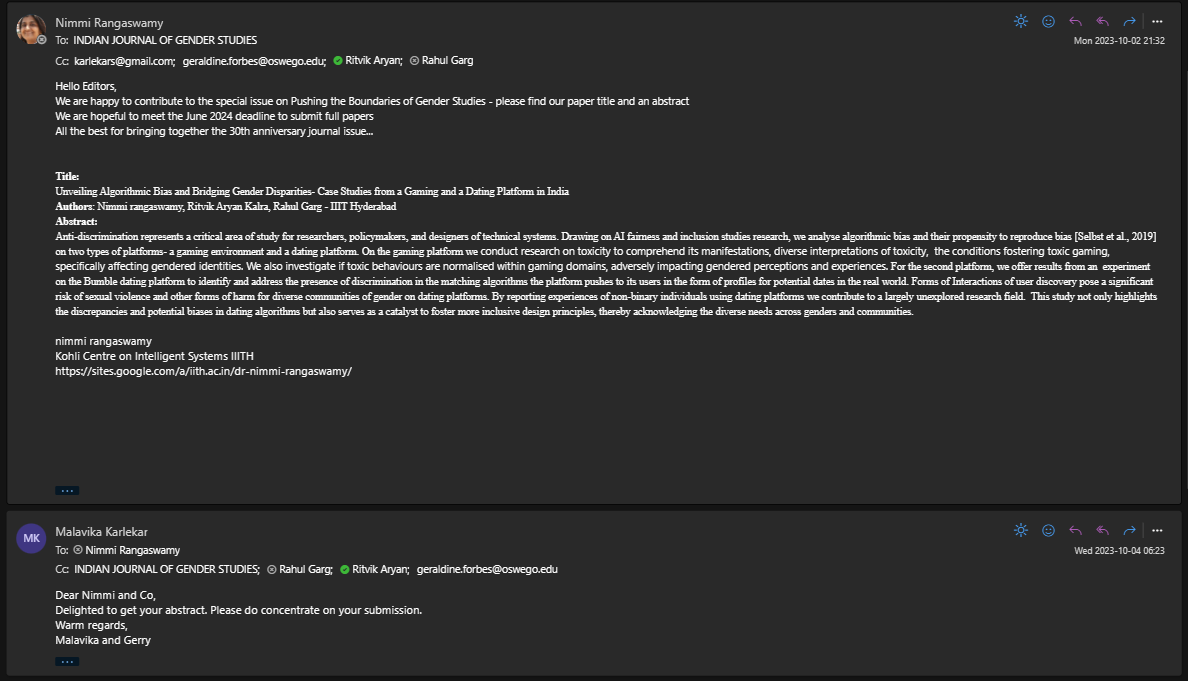
\includegraphics[scale=0.5]{figures/Supplimentary Material/Journal Paper Acceptance.png}
 \caption{Mail from the editors of Indian Journal of Gender Studies (IJGS), accepting our abstract submission for the paper.}
 \label{fig:img6}
\end{figure}

\begin{figure}[h]
 \centering
 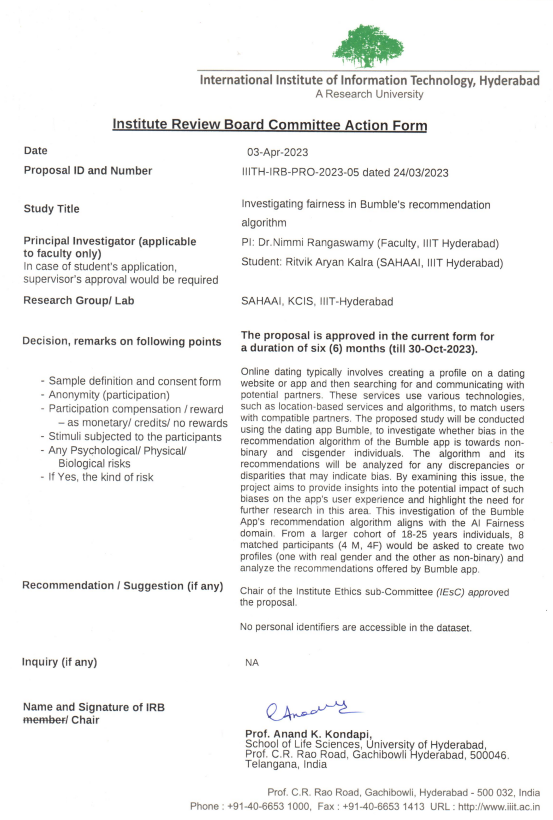
\includegraphics[scale=0.8]{figures/Supplimentary Material/Ethics Board Apporval.png}
 \caption{Approval Letter from the Ethics Board of the International Institute of Information Technology, Hyderabad, for conducting the study.}
 \label{fig:img7}
\end{figure}

\section*{Reviews, for the paper Exploring Gender Disparities in Bumble's Match Recommendations}
\subsection*{Review 1}

\textbf{SCORE:} 1 (Weak Accept)

\textbf{Contextual Background:} The study could benefit from a more detailed historical backdrop of online dating in India. Understanding the evolution of dating platforms in the region might add layers to the research.

\textbf{Comparison with Other Studies:} Briefly highlighting how this research differs from other similar studies would set the stage better.

\textbf{Literature Review Depth:} While interdisciplinary, the literature review might gain from a more exhaustive exploration of each discipline, possibly citing more recent or region-specific studies.

\textbf{Technological Aspects:} Since Bumble is a technology platform, a deeper dive into its technical specifications or how its algorithm is fundamentally designed would be beneficial.

\textbf{Method Validation:} The research should ensure that the methodologies employed, especially concerning fictitious profiles, are validated against established research standards or benchmarks.

\textbf{Confounding Variables:} The study needs to address potential confounding variables that could impact the observed disparities. This would include user behavior, historical data, and the inherent biases of the users themselves.

\textbf{User Feedback:} Alongside quantitative data, user feedback or testimonials would add a layer of real-world context to the findings.

\textbf{Recommendations' Feasibility:} While making suggestions, it would be pertinent to explore their feasibility, especially from a technological and business perspective for platforms like Bumble.

\textbf{Comparative Analysis:} A comparative analysis with other dating apps popular in India might provide a broader picture of the industry's landscape.

\textbf{Future Scope:} Addressing the potential future scope of the study or suggesting areas for subsequent research can make the research more forward-looking.

\textbf{Stakeholder Perspective:} It might be insightful to include perspectives from other stakeholders, like app developers, tech ethicists, or even Bumble's official stance on the findings.

By addressing these elements, the study can present a more holistic, comprehensive, and actionable view on gender disparities in digital dating platforms in the Indian context.
Literature review should be updated.

\subsection*{Review 2}

\textbf{SCORE:} 1 (Weak Accept)

\textbf{Introduction and Context:} This study falls short in providing a comprehensive background of the online dating scenario in India. A deeper historical analysis would lend more credence and foundation to the work.

\textbf{Distinguishing the Work:} The research does not effectively differentiate itself from existing studies. It's crucial to showcase what sets this study apart in the vast domain of online dating research.

\textbf{Literature Review:} The interdisciplinary approach, while admirable, feels lacking in depth. Each domain should be explored with greater emphasis, especially focusing on the most recent developments and India-centric studies.

\textbf{Technical Insights:} For a study concentrating on Bumble, there's a surprising lack of technical dissection. It's imperative to discuss the app's core algorithmic aspects for a more well-rounded understanding.

\textbf{Research Techniques:} Some methodologies, notably the use of fictitious profiles, need to be cross-verified with standardized research norms to ensure credibility.

\textbf{Interplay of Variables:} The study appears to gloss over potential external factors that might affect the findings, such as user preferences, historical patterns, or ingrained user biases.

\textbf{Real-world Evidence:} The data lacks a human touch. Direct testimonials or feedback would have enriched the findings, making them more relatable.

\textbf{Practicality of Suggestions:} The proposed recommendations don't seem to consider the practical limitations or challenges from Bumble's perspective. This oversight can affect the study's applicability.

\textbf{Market Analysis:} The absence of a comparative study with other prominent Indian dating apps feels like a missed opportunity. Such a comparison would offer valuable industry insights.

\textbf{Forward Thinking:} The research could benefit from a section focusing on potential future developments or areas ripe for further investigation.

\textbf{Voices from the Field:} The research would be more grounded if it incorporated viewpoints from related stakeholders – like app developers or industry specialists. An official statement or perspective from Bumble would also lend authenticity.

\textbf{Concluding Remarks:} The study provides an insightful look into the gender dynamics on Bumble, but it has areas that need polishing. An update in literature and a more robust research approach would significantly elevate its quality.